\section{Phân tích vấn đề:}
\subsection{Problem Statement:}
Học sinh/ sinh viên mất đi động lực khi đối mặt với việc học các chương trình ngữ pháp khô khan, từ vựng khó nhớ, dẫn đến thiếu ứng dụng và kém tiến bộ trong quá trình học ngôn ngữ; vì vậy cần 1 hệ thống RPG tích hợp AI để biến quá trình học tiếng Anh như một trò chơi giải trí, giúp tăng sự hứng thú và ghi nhớ dài hạn thông qua tương tác cốt truyện.

\subsection{Các bên liên quan (Stakeholder):}


\begin{table}[H]
\centering
\caption{Bảng Stakeholder}
\renewcommand{\arraystretch}{1.5} % Giúp các hàng dãn ra cho dễ đọc
\begin{tabularx}{\textwidth}{|>{\raggedright\arraybackslash}p{2.5cm}|>{\raggedright\arraybackslash}p{2.5cm}|X|>{\centering\arraybackslash}p{1.5cm}|>{\centering\arraybackslash}p{1.8cm}|}
\hline
\textbf{Stakeholder} & \textbf{Vai trò} & \textbf{Nhu cầu/mong đợi} & \textbf{Ảnh hưởng} & \textbf{Mức độ quan trọng} \\ \hline
Sinh viên & Người dùng cuối & Game mượt, từ vựng sát thực tế, cảm giác "lên trình" tiếng Anh qua các chỉ số (level, rank). & Cao & Cao \\ \hline
Nhóm phát triển & Đội ngũ thực thi & Quy trình code rõ ràng, tài liệu đầy đủ, không bị chồng chéo nhiệm vụ. & Cao & Cao \\ \hline
Giảng viên hướng dẫn & Người đánh giá & Áp dụng đúng đắn các quy tắc, công thức tư duy của môn học, báo cáo đúng tiến độ công việc. & Trung bình & Cao \\ \hline
Nhà cung cấp AI & Đối tác hạ tầng & API ổn định, chi phí thấp (hoặc miễn phí), phản hồi nhanh. & Thấp & Trung bình \\ \hline
Người yêu thích game/RPG & Người dùng mở rộng & Cốt truyện hấp dẫn, cơ chế chơi độc đáo, tương tác với NPC thú vị. & Thấp & Thấp \\ \hline
\end{tabularx}
\end{table}

\subsection{Phạm vi bài toán (Scope):}
\subsubsection{Trong phạm vi (In-scope):}

\begin{table}[H]
\centering
\renewcommand{\arraystretch}{1.5}
\begin{tabularx}{\textwidth}{|>{\raggedright\arraybackslash}p{3.5cm}|X|>{\raggedright\arraybackslash}p{4cm}|}
\hline
\textbf{Nội dung} & \textbf{Chi tiết thực hiện} & \textbf{Ghi chú} \\ \hline
Chức năng phát triển & - Hệ thống hội thoại AI (Text-based) để học từ vựng/ngữ pháp. \newline - Cơ chế của game nhập vai: Thu thập vật phẩm, tăng cấp (Level up), bảng chỉ số (Stats). \newline - Hệ thống nhiệm vụ (Quests) dựa trên các bài tập & \textbf{Phân rã:} Chia nhỏ thành các Module độc lập để mọi người trong nhóm có thể code song song \\ \hline
Đối tượng phục vụ & Sinh viên đại học (đặc biệt là khối không chuyên Anh) muốn cải thiện vốn từ vựng và kỹ năng đọc hiểu thông qua giải trí & \textbf{Trừu tượng hóa:} Chỉ tập trung vào nhu cầu "Học mà chơi", lược bỏ các tính năng mạng xã hội phức tạp \\ \hline
Địa điểm/Phạm vi & Triển khai dưới dạng ứng dụng Web hoặc Mobile (hoặc cả hai). Phục vụ trong môi trường học tập cá nhân. & \textbf{Nhận dạng mẫu:} Sử dụng cấu trúc Client-Server phổ biến để dễ dàng quản lý mã nguồn trên GitHub. \\ \hline
Thời gian thực hiện & Khoảng 10 tuần (Từ giai đoạn lên ý tưởng đến khi Demo sản phẩm cuối cùng). & \textbf{Thuật toán:} Phân bổ thời gian theo sơ đồ Gantt để tối ưu hóa năng suất nhóm. \\ \hline
\end{tabularx}
\end{table}

\subsubsection{Ngoài phạm vi (Out-of-scope):}

\begin{table}[H]
\centering
\renewcommand{\arraystretch}{1.5}
\begin{tabularx}{\textwidth}{|>{\raggedright\arraybackslash}p{3.5cm}|X|>{\raggedright\arraybackslash}p{4cm}|}
\hline
\textbf{Tính năng/hạng mục} & \textbf{Lý do loại trừ} & \textbf{Khả năng phát triển sau này} \\ \hline
Luyện nói (Speaking) và Luyện nghe (Listening) & Độ phức tạp: Đòi hỏi tích hợp Speech-to-Text và xử lý âm thanh phức tạp, dễ gây lỗi trễ (latency). & Rất khó có khả năng (chỉ tính đến khi và chỉ khi giai đoạn 2.0 sau khi ổn định Reading/Vocab). \\ \hline
Đồ họa 3D / Thế giới mở & Thời gian và Kỹ năng: Nhóm 6 người làm trong khoảng 10 tuần thì không đủ nguồn lực để làm Animation 3D mượt mà. & Có thể nâng cấp đồ họa, nhưng không ưu tiên bằng Logic học tập. \\ \hline
Chế độ chơi nhiều người (Multiplayer) & Kỹ thuật: Cần quản lý Server, Database thời gian thực và giải quyết vấn đề đồng bộ hóa. & Có (Dưới dạng bảng xếp hạng - Leaderboard đơn giản). \\ \hline
Hệ thống thanh toán / Thương mại hóa & Ngân sách và Pháp lý: Dự án tập trung vào học thuật và giải quyết vấn đề tư duy tính toán, không phải kinh doanh. & Không ưu tiên. \\ \hline
\end{tabularx}
\end{table}

\subsection{Phân tích hiện trạng (AS-IS process):}
\subsubsection{Sơ đồ quy trình hiện tại:}

\noindent \textbf{Sơ đồ quy trình hiện tại (flowchart):} \medskip
\begin{figure}[H]
    \centering
    
\includegraphics[width=0.8\textwidth]{flowchart.png}
    \caption{Sơ đồ quy trình AS-IS hiện tại}
    \label{fig:as_is_flowchart}
\end{figure}

\vspace{1em} % Tạo khoảng cách giữa ảnh và tiêu đề bảng tiếp theo
\noindent \textbf{Quy trình AS - IS process chi tiết:} \smallskip

\begin{table}[H]
\centering
\small
\renewcommand{\arraystretch}{1.6}
\begin{tabularx}{\textwidth}{|c|>{\raggedright\arraybackslash}p{3cm}|X|>{\centering\arraybackslash}p{2.5cm}|}
\hline
\textbf{Bước} & \textbf{Tên hoạt động thực tế} & \textbf{Mô tả chi tiết (Góc nhìn thuật toán)} & \textbf{Thời gian ước tính} \\ \hline
1 & Bắt đầu phiên học & \texttt{Initialize\_Session()}: Sinh viên thiết lập môi trường (mở giáo trình, tìm bài đọc, chuẩn bị giấy bút). & 5 phút \\ \hline
2 & Đọc đoạn văn (Reading) & \texttt{While not End\_of\_Text}: Bắt đầu tiến trình đọc hiểu. Bộ não xử lý thông tin. & 15 - 20 phút \\ \hline
3 & Dừng lại \& Tra cứu & \texttt{IF gặp\_từ\_mới == True}: Kích hoạt hàm ngắt mạch. Sinh viên rời mắt khỏi bài đọc, mở điện thoại hoặc từ điển để tra nghĩa. & 10 - 15 phút (cộng dồn) \\ \hline
4 & Chép từ & \texttt{Save\_to\_Local()}: Ghi chép từ vựng và nghĩa tiếng Việt ra vở một cách thủ công. Sau đó quay lại Bước 2. & 5 - 10 phút (cộng dồn) \\ \hline
5 & Làm bài tập & \texttt{Execute\_Task()}: Khi \texttt{Hết\_đoạn\_văn == True}, chuyển sang làm các bài tập trắc nghiệm dựa trên trí nhớ ngắn hạn. & 15 - 20 phút \\ \hline
6 & Kiểm tra đáp án & \texttt{Validate\_Results()}: Lật cuối sách xem đáp án hoặc đợi giáo viên chữa. Độ trễ phản hồi cao khiến não khó liên kết lỗi sai. & 5 - 10 phút \\ \hline
7 & Chữa bài tập \& Tự ôn tập & \texttt{Error\_Correction()} \& \texttt{Rote\_Memorization()}: Lập danh sách lỗi và học thuộc lòng từ vựng không có ngữ cảnh tương tác. & 10 phút \\ \hline
8 & Kết thúc phiên học & \texttt{End\_Session()}: Output trả về là "Ghi nhớ ngắn hạn" và trạng thái tâm lý "Thiếu động lực". & - \\ \hline
\multicolumn{3}{|r|}{\textbf{Tổng thời gian học dự kiến}} & \textbf{65 - 90 phút} \\ \hline
\end{tabularx}
\end{table}

\begin{enumerate}
\item Điểm nghẽn (Bottlenecks):
\begin{enumerate}[label=\alph*), nosep]
    \item \textbf{Điểm nghẽn 1: Sự gián đoạn ngữ cảnh:} Sinh viên liên tục phải chuyển đổi trạng thái giữa việc "Đọc hiểu" và "Tra từ điển". Điều này phá vỡ luồng tập trung  và làm giảm tốc độ xử lý thông tin.
    \item \textbf{Điểm nghẽn 2: Vòng lặp phản hồi trễ:} Khi làm sai sinh viên chỉ biết đáp án đúng là gì chứ không được giải thích tại sao sai ngay tại thời điểm đó (trừ khi có gia sư).
    \item \textbf{Điểm nghẽn 3: Ghi nhớ cơ học:} Việc chép từ vựng ra vở thiếu tính lặp lại, gây ngắt quãng và thiếu cảm xúc/tương tác, dẫn đến tỷ lệ rụng rớt thông tin rất cao.
\end{enumerate}


\item Tồn tại:
\begin{enumerate}[label = \alph*), nosep]
	\item \textbf{Thiếu động lực:} Quá trình học tiếng Anh mang tính "tuyến tính" và khô khan. Sinh viên không có phần thưởng ngay lập tức để duy trì hứng thú học tập.
	\item \textbf{Hiệu suất kém:} Dành ra nhiều tiếng đồng hồ nhưng lượng từ vựng thực sự đọng lại ở Trí nhớ dài hạn rất thấp do các từ này không được đặt trong các tình huống ứng dụng thực tế.
\end{enumerate}

\end{enumerate}

\subsubsection{Giải pháp hiện có trên thị trường}

Khi đánh giá về các giải pháp tiêu biểu hiện nay trên thị trường, có ba nhóm chính đó là:

\begin{itemize}
    \item \textbf{Nhóm 1:} App học truyền thống có yếu tố kết hợp trò chơi cho người dùng tương tác (Gamification): Duolingo, Memrise.
    \item \textbf{Nhóm 2:} Chatbot AI phổ biến hiện nay: ChatGPT Voice, Character.ai, Replika, v.v.
    \item \textbf{Nhóm 3:} Những game RPG hoàn toàn bằng tiếng Anh: Genshin Impact, Persona, v.v.
\end{itemize}

\begin{table}[H]
\centering
\caption{Bảng đánh giá các điểm mạnh, điểm yếu của ba nhóm sản phẩm hỗ trợ học tiếng Anh}
\label{tab:danh-gia-giai-phap}
\small
\begin{tabularx}{\textwidth}{|l|X|X|X|}
\hline
\textbf{Giải pháp} & \textbf{Điểm mạnh} & \textbf{Điểm yếu} & \textbf{Bài học rút ra} \\ \hline
\textbf{Nhóm 1} & 
\begin{itemize}[leftmargin=*, nosep]
    \item Giao diện bắt mắt, tính năng trò chơi hóa (streak, bảng xếp hạng) giữ chân người dùng tốt.
    \item Có thuật toán lặp lại ngắt quãng (Spaced Repetition) giúp ghi nhớ dài hạn.
\end{itemize} & 
\begin{itemize}[leftmargin=*, nosep]
    \item Thiếu ngữ cảnh: Các câu ví dụ thường rời rạc, máy móc.
    \item Không có tính nhập vai (Role-play), người dùng tương tác thụ động.
\end{itemize} & 
\begin{itemize}[leftmargin=*, nosep]
    \item Phát triển hệ thống Quest (Nhiệm vụ): Dùng LLM tạo nhiệm vụ dựa trên ngữ cảnh game thay vì dịch câu rời rạc.
    \item Giữ lại Spaced Repetition để ôn tập từ mới sau mỗi nhiệm vụ.
\end{itemize} \\ \hline

\textbf{Nhóm 2} & 
\begin{itemize}[leftmargin=*, nosep]
    \item Giao tiếp tự nhiên, ngữ cảnh mở.
    \item Phản hồi thời gian thực, hỗ trợ nhập liệu bằng giọng nói (Speech-to-text).
\end{itemize} & 
\begin{itemize}[leftmargin=*, nosep]
    \item Thiếu định hướng học tập: Không có lộ trình độ khó tăng dần.
    \item Không tự động lưu trữ và phân tích lỗi sai có hệ thống.
\end{itemize} & 
\begin{itemize}[leftmargin=*, nosep]
    \item Tích hợp vào Game các xử lý logic: thêm FastAPI xử lý logic để trích xuất từ vựng (Vocabulary extraction) và sửa lỗi ngữ pháp (Grammar correction) ngầm, sau đó lưu vào Firebase.
\end{itemize} \\ \hline

\textbf{Nhóm 3} & 
\begin{itemize}[leftmargin=*, nosep]
    \item Ngữ cảnh giao tiếp thực tế đa dạng, động lực chơi cao, thu hút người dùng.
\end{itemize} & 
\begin{itemize}[leftmargin=*, nosep]
    \item Rào cản ngôn ngữ lớn: Độ khó của ngữ pháp, từ vựng mà không có dịch nghĩa của ngôn ngữ mẹ đẻ sẽ khiến người mới học sẽ bị ngợp, nản chí và dẫn đến bỏ cuộc.
\end{itemize} & 
\begin{itemize}[leftmargin=*, nosep]
    \item Tích hợp vào Game các chế độ khó tùy chọn (Adaptive difficulty)
    \item Xây dựng rule để LLM điều chỉnh từ vựng của NPC dựa trên hồ sơ lỗi của người chơi. Từ vựng nào còn yếu, sai nhiều sẽ xuất hiện nhiều hơn.
\end{itemize} \\ \hline
\end{tabularx}
\end{table}
→ Các giải pháp hiện tại hoặc là \textbf{quá thiên về học thuật, thiếu bối cảnh} (Duolingo), hoặc là \textbf{quá tự do, thiếu cấu trúc sư phạm} (Chatbot AI). Mục tiêu của dự án sẽ là trung hòa các điểm mạnh của các giải pháp trên và hạn chế các điểm yếu hiện hữu.

\subsubsection{Phân tích SWOT}
\begin{enumerate}
\item Strengths (Điểm mạnh của tổ chức/đơn vị): \newline
- Nhân sự: nhóm với 6 người giúp khối lượng công việc dễ dàng được phân chia, hiệu suất làm việc tối ưu nhất. \newline
- Ứng dụng các công nghệ phổ biến có tính ứng dụng cao như: AI tạo đoạn hội thoại, tính năng nhắc nhở ôn tập từ vựng. \newline
- Trải nghiệm mới mẻ: học tiếng Anh thông qua việc giao tiếp, tương tác với nhân vật trong Game thay vì các dạng câu hỏi bài tập truyền thống dễ gây nhàm chán.

\item Weaknesses (Điểm yếu): \newline
- Cần ưu tiên những tính năng cốt lõi nhất, tránh việc cố làm quá nhiều tính năng dẫn đến việc Game không đạt được yêu cầu tương tác với người dùng. \newline
- Cần nhiều thời gian để các thành viên tự tìm hiểu và ghép nối các công nghệ mới lại với nhau. \newline
- Việc sử dụng các dịch vụ AI của bên thứ ba (LLM,API trả lời câu hỏi) thường bị giới hạn lượt dùng miễn phí hoặc có thể phát sinh chi phí khi nhóm thử nghiệm liên tục.

\item Opportunities (Cơ hội): \newline
- Tiềm năng phát triển: Giải quyết đúng nhu cầu thực tế của sinh viên (ngại giao tiếp tiếng Anh). Sản phẩm hoàn thiện có thể làm điểm nhấn giá trị trong CV xin việc hoặc tham gia các cuộc thi công nghệ. \newline
- Tài nguyên hỗ trợ dồi dào: Hiện nay có rất nhiều thư viện lập trình, mã nguồn mở và tài liệu về AI/Game được chia sẻ miễn phí, giúp tiết kiệm thời gian xây dựng từ đầu. \newline


\item Threats (Thách thức): \newline
- Rủi ro vận hành khi báo cáo: Sản phẩm phụ thuộc nhiều vào kết nối mạng và tốc độ phản hồi của server AI. Nếu đường truyền mạng yếu hoặc server lỗi lúc demo, trải nghiệm sẽ bị gián đoạn. \newline
- Rủi ro tiến độ: Dự án có nhiều thành phần liên kết chặt chẽ (người làm giao diện game phải đợi người làm dữ liệu AI). Nếu một khâu bị chậm trễ sẽ kéo theo toàn bộ tiến độ của nhóm bị ảnh hưởng. \newline
- Tính ổn định của sản phẩm: So với các đề tài an toàn khác, việc AI tự sinh câu trả lời có nguy cơ phát sinh nhiều lỗi (bug) không lường trước được trong quá trình chạy thực tế.
\end{enumerate}

\subsection{Các điểm đau của người dùng (Paint Points):}
Link phỏng vấn sâu (5 người):
\url{https://docs.google.com/forms/d/e/1FAIpQLSe44wZf9WbY6Nu-zK6tJdWbus8pBflSfa5TZw3yNxYk3n1DjQ/viewform?usp=header} \newline
\newcommand{\redcircle}{\textcolor{red}{$\bullet$}}
\newcommand{\yellowcircle}{\textcolor{yellow}{$\bullet$}}


\renewcommand{\arraystretch}{1.5} % Giúp các hàng có khoảng thở, không bị dính chữ

\begin{table}[H]
\centering
\caption{Bảng tổng hợp các điểm đau (Pain points) từ khảo sát người dùng}
\label{tab:pain-points}
\footnotesize % Chuyển xuống size này để bảng dễ thở hơn trên khổ giấy A4
\begin{tabularx}{\textwidth}{|c|>{\hsize=0.8\hsize}X|>{\hsize=1.2\hsize}X|c|c|c|}
\hline
\textbf{STT} & \textbf{\makecell{Pain point\\từ khảo sát}} & \textbf{Mô tả chi tiết} & \textbf{\makecell{Mức độ\\nghiêm\\trọng}} & \textbf{\makecell{\% Người\\gặp phải}} & \textbf{Tần suất} \\ \hline

1 & \redcircle Thiếu người sửa lỗi và giải thích cặn kẽ. & Người dùng không hài lòng khi các công cụ (Grammarly, Study4, sách ngữ pháp) "chỉ hiện dấu tích xanh/đỏ hoặc cung cấp đáp án đúng chứ không giải thích lý do đằng sau". Việc tự mày mò nguyên nhân tốn nhiều thời gian, ngại hỏi bạn bè nên lỗi sai dần trở thành thói quen không sửa được. & 5 & 56,5\% & Hằng ngày \\ \hline

2 & \redcircle  Áp lực đánh giá, "bí từ" khi ghép câu. & Có ý tưởng bằng tiếng Việt nhưng khi cần tự viết câu (nhắn tin, viết email, tham gia seminar Zoom) thì lúng túng, e ngại cách diễn đại không đúng chuẩn dẫn đến việc tốn thời gian vô ích. & 4 & 47,8\% & Hằng tuần \\ \hline

3 & \redcircle  Học thụ động, thiếu môi trường thực hành. & Việc ghi chép flashcard (Anki, sổ tay) hay học app (Duolingo) bị đánh giá là thụ động và rời rạc. Người được khảo sát cảm thấy các ví dụ quá máy móc, không có ngữ cảnh thực tế. Vì học chay và không có môi trường thực hành dẫn đến việc phản ứng chậm trong các tình huống thực tế. & 4 & 43,5\% & Hằng ngày \\ \hline

4 & \yellowcircle Phương pháp học nhàm chán, rập khuôn. & Việc học bằng flashcard hay chọn đáp án A, B, C, D có sẵn trên app bị lặp đi lặp lại mà không có sự sáng tạo mới mẻ, gây ra chán nản và làm cho người học dễ bỏ cuộc. Người học cần một thế giới tương tác, có mục tiêu rõ ràng, sử dụng tiếng Anh làm công cụ để vượt qua thử thách. & 3 & 39,1\% & Hằng ngày \\ \hline

\end{tabularx}
\end{table}

\subsection{Kiểm chứng điểm đau (Pain Point Validation)}
\subsubsection{Kết quả khảo sát:}
Dữ liệu khảo sát được thu thập từ nhóm đối tượng mục tiêu là \textbf{sinh viên đại học (độ tuổi 18–22), chủ yếu không chuyên tiếng Anh}, thông qua biểu mẫu trực tuyến. Nhóm người học này có đặc điểm chung là đã có nền tảng cơ bản nhưng gặp nhiều khó khăn trong việc sử dụng tiếng Anh trong thực tế. \newline
\textbf{Biểu đồ thống kê (Data Visualization)}
\begin{figure}[H]
    \centering
    
\includegraphics[width=0.8\textwidth]{cau5.png}
    \label{fig:cau5}
\end{figure}

\begin{figure}[H]
    \centering
    
\includegraphics[width=0.8\textwidth]{cau1.png}
    \label{fig:cau1}
\end{figure}

\begin{figure}[H]
    \centering
    
\includegraphics[width=0.8\textwidth]{cau3.png}
    \label{fig:cau3}
\end{figure}

\begin{figure}[H]
    \centering
    
\includegraphics[width=0.8\textwidth]{cau6.png}
    \label{fig:cau6}
\end{figure}

\begin{figure}[H]
    \centering
    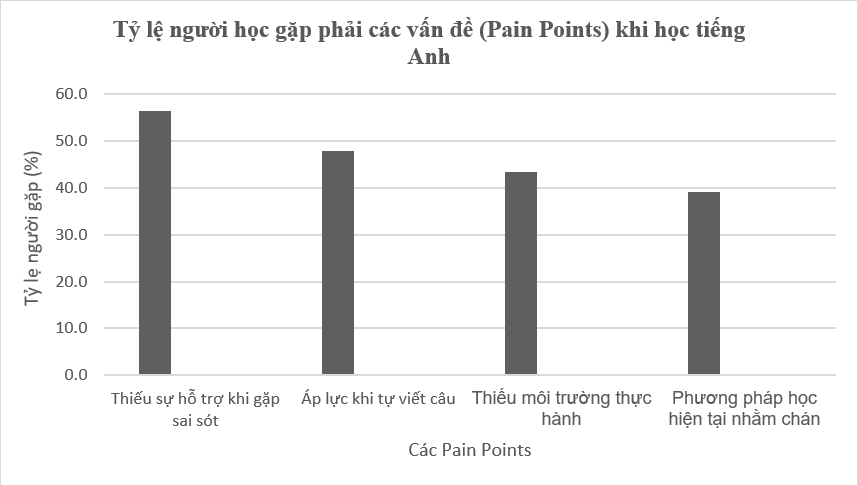
\includegraphics[width=0.8\textwidth]{tyle.png}
    \label{fig:tyle}
\end{figure}

Các biểu đồ được sử dụng nhằm trực quan hóa:
\begin{itemize}[leftmargin = *, nosep]
\item Tỷ lệ người học gặp phải các vấn đề phổ biến. 
\item Mức độ xuất hiện của từng pain point.
\item Xu hướng và hành vi học tập của người tham gia khảo sát.
\end{itemize}
\textbf{Số liệu cụ thể từ khảo sát:} \newline

Kết quả khảo sát cho thấy nhiều vấn đề đáng chú ý trong quá trình học Tiếng Anh của người học: \newline
\begin{itemize}[leftmargin = *, nosep]
\item Khoảng \textbf{56.5\%} người tham gia cho biết họ gặp khó khăn trong việc \textbf{thiếu phản hồi và sửa lỗi theo thời gian thực}. Điều này cho thấy phần lớn người học không có cơ chế kiểm tra và điều chỉnh sai sót ngay khi sử dụng ngôn ngữ. 

\item \textbf{47.8\%} người học cảm thấy \textbf{áp lực khi tự viết câu}, dẫn đến sự thiếu tự tin trong việc diễn đạt ý tưởng bằng tiếng Anh. Đây là một rào cản lớn đối với việc phát triển kỹ năng chủ động (productive skills). 

\item \textbf{43.5\%} cho rằng họ \textbf{thiếu môi trường thực hành thực tế}, khiến việc học trở nên rời rạc và khó áp dụng vào tình huống giao tiếp thực tế. 

\item Bên cạnh đó, \textbf{39.1\%} người học nhận định rằng \textbf{phương pháp học hiện tại mang tính lặp lại và thiếu tính hấp dẫn}, dẫn đến giảm động lực học tập theo thời gian.

\end{itemize}

\begin{itemize}[leftmargin = *, nosep]
    \item \textbf{Độ tuổi:} Chủ yếu từ 18 đến 22
    \item \textbf{Trình độ tiếng Anh:} Từ cơ bản (Beginner) đến trung cấp (Intermediate)
    \item \textbf{Hình thức học tập phổ biến:}
    \begin{itemize}
        \item Sử dụng các ứng dụng học tiếng Anh.
        \item Học qua flashcard.
        \item Tự học bằng giáo trình.
    \end{itemize}
\end{itemize}
Những đặc điểm này phản ánh một nhóm người học có khả năng tiếp cận tài nguyên học tập đa dạng, nhưng vẫn gặp khó khăn trong việc chuyển hóa kiến thức thành kỹ năng sử dụng thực tế. \newline

\textbf{Nhận xét tổng quan:}
Từ các dữ liệu thu thập được, có thể nhận thấy rằng vấn đề cốt lõi không nằm ở việc thiếu tài liệu học tập, mà nằm ở \textbf{cách thức học và môi trường học chưa phù hợp}. \newline
Cụ thể:
\begin{itemize}[leftmargin = *, nosep]
\item Việc học còn thiếu \textbf{tính tương tác hai chiều}
\item Thiếu \textbf{ngữ cảnh thực tế để áp dụng kiến thức}
\item Thiếu \textbf{phản hồi tức thời để điều chỉnh sai sót}
\end{itemize}

Hệ quả là người học thường rơi vào trạng thái: \newline
=> \textbf{“Biết lý thuyết nhưng lại không thể sử dụng được”}

\subsubsection{Top 3 Pain Points quan trọng nhất}
Dựa trên các tiêu chí: \textbf{Mức độ nghiêm trọng (Severity), Tần suất (Frequency), Tỷ lệ người gặp (Impact)}.

\begin{description}
    \item[Pain Point \#1: Thiếu phản hồi \& sửa lỗi theo thời gian thực] \hfill \\
    \textit{Lý do ưu tiên:} 
    \begin{itemize}[nosep]
        \item Mức độ nghiêm trọng cao nhất (5/5).
        \item Tỷ lệ gặp cao nhất (56.5\%).
    \end{itemize}
    \textbf{Phân tích:} Đây là vấn đề nổi bật nhất với tỷ lệ người gặp cao nhất. Việc không nhận được phản hồi ngay lập tức khiến người học không thể nhận diện và sửa lỗi kịp thời, dẫn đến việc lặp lại sai sót trong thời gian dài.

    \item[Pain Point \#2: Áp lực khi tự viết câu, thiếu tự tin] \hfill \\
    \textit{Lý do ưu tiên:} 
    \begin{itemize}[nosep]
        \item Ảnh hưởng trực tiếp đến kỹ năng sử dụng ngôn ngữ (Active skill).
    \end{itemize}
    \textbf{Phân tích:} Người học thường gặp khó khăn khi chuyển từ việc “hiểu” sang “sử dụng” ngôn ngữ. Áp lực khi viết hoặc nói khiến họ ngại thực hành, từ đó hạn chế sự phát triển của kỹ năng giao tiếp.

    \item[Pain Point \#3: Học thụ động, thiếu môi trường thực hành] \hfill \\
    \textit{Lý do ưu tiên:} 
    \begin{itemize}[nosep]
        \item Xuất hiện thường xuyên trong quá trình học hàng ngày.
    \end{itemize}
    \textbf{Phân tích:} Phần lớn phương pháp học hiện tại mang tính thụ động, thiếu ngữ cảnh thực tế. Điều này làm giảm khả năng ghi nhớ và khiến người học khó áp dụng kiến thức vào các tình huống thực tế.
\end{description}

\subsubsection{Trích dẫn từ người dùng (Quotes)}
Một số phản hồi tiêu biểu từ khảo sát:

\begin{itemize}
    \item \textit{“Mình tra từ xong nhưng không biết dùng trong câu như thế nào.”}
    \item \textit{“Làm sai mà không ai giải thích nên không biết sửa.”}
    \item \textit{“Học từ vựng nhiều nhưng gặp tình huống thật lại không dùng được.”}
    \item \textit{“Học app thì vui lúc đầu, nhưng sau đó rất chán vì lặp lại.”}
\end{itemize}

\vspace{10pt}
\textbf{Insight chính:} \\
Từ các dữ liệu định lượng và định tính, có thể rút ra insight cốt lõi: \\
\fbox{
    \parbox{0.95\textwidth}{
        \centering \textbf{=> Người học không chỉ cần một công cụ cung cấp kiến thức, mà cần một hệ thống có khả năng tương tác, phản hồi và đặt họ vào ngữ cảnh sử dụng thực tế.}
    }
}